\documentclass{beamer}
\usepackage{graphicx}
\usefonttheme[onlymath]{serif}
\usepackage[utf8]{inputenc}
\renewcommand{\vec}[1]{\mathbf{#1}}
 \newcommand{\grad}{\nabla}
\newcommand{\partiald}[2]{\frac{\partial {#1} }{\partial {#2}}}
%Information to be included in the title page:
\title{Rossby Waves}
\author{Sam Harrison}
\institute{MPE CDT }
\date{\today}
 
 
 
\begin{document}
 
\frame{\titlepage}
  
\begin{frame}
\frametitle{Shallow Water Equations}
Starting from the equations:
\begin{align}
\frac{\partial \vec{u}}{\partial t}+(\vec{u}\cdot\nabla) \vec{u}+f\vec{\hat{z}}\times\ \vec{u}& =-g\grad h\label{mom}\\
\frac{\partial h}{\partial t}+\grad\cdot(h\vec{u})& =0\label{heq}
\end{align}
%Equation \eqref{mom} comes from navier Stokes
%n the shallow water equations we assume that the height of the displacement is small compared to the height of the fluid and also the motion is 2d. 
If we consider small amplitude motions on the surface $h=H+\eta$, $\vec{u}=(u',v',0)$ where $\eta<<0,\;u',v'<<0$.
Looking at the $O(1)$ terms, we get these equations.
\begin{align}
\partiald{u'}{t}-fv'&=-g\partiald{\eta}{x}\label{x}\\
\partial{v'}{t}+fu'&=-g\partiald{\eta}{y}\label{y}\\
\partiald{\eta}{t}+H\partiald{u'}{x}+H\partiald{v'}{y}&=0 \label{h}
\end{align}
\end{frame}
\begin{frame}
\frametitle{Gravity Waves}
The simplest case of the shallow water equations is in the absence of rotation $(f=0)$. If we then take $\partiald{\eqref{x}}{x},\; \partiald{\eqref{y}}{y},\;\partiald{\eqref{h}}{t}$, we get the wave equation
\begin{align}
\partiald{^2\eta}{t^2}-gH\grad^2\eta=0\label{wave}
\end{align}
This is the wave equation so will have solutions of the form.
\begin{align}
\eta=h_0\exp(i(kx+\ell y+\omega t))\label{wavepacket}
\end{align}
which by plugging this into Equation \eqref{wave}, we get the dispersion relation

\begin{align}
\omega=\pm\sqrt{gH(k^2+\ell^2)}
\end{align}
\end{frame}

\begin{frame}
\frametitle{Inertio-Gravity/ Poincaré waves}
Now looking at the case where we have constant rotation $(f=f_0)$
By taking various partial derivatives of Equations \eqref{x}, \eqref{y}, \eqref{h}, we obtain the equation.
\begin{align}
\partiald{}{t}\left(\partiald{^2}{t^2}+f_0^2-gH\grad^2\right)\eta=0
\end{align}
Which when we plug in \eqref{wavepacket} gives us the dispersion relation
\begin{align}
-i\omega(-\omega^2+gH(k^2+\ell^2)+f_0^2)
\end{align}
So has solutions
\begin{align}
\omega=0 && \mathrm{or} && \omega=\pm\sqrt{f_0^2+gH(k^2+\ell^2)}
\end{align}
The zero frequency case is the time independent flow. The flow here oscillates at greater frequency than the standard gravity waves.

\end{frame}
\begin{frame}
\frametitle{Comparing Shallow Water Waves}
\centering\includegraphics[scale=0.25]{"Shallow Water Waves"}

\end{frame}
 \begin{frame}
 \frametitle{Quasi stationary synoptic Rossby waves high amplitude during weather events }
\framesubtitle{by Petoukhov, Rahmstorf, Pteri and Schellnhuber 2013}
\begin{itemize}
	\item Investigated physical model of quasi resonance effect.
	\item Forced wave trapping a free wave.
	\item Amplification of pressure system.
	\item Extreme weather results.
\end{itemize}
\centering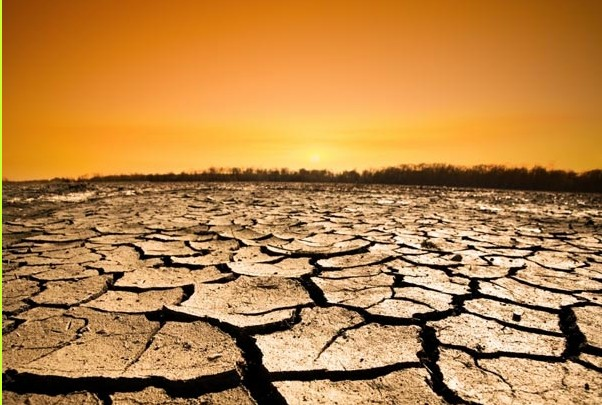
\includegraphics[height=0.4\textheight]{drought}

\end{frame}
\begin{frame}
\frametitle{Amplified mid-latitude planetary waves favour particular regional weather extremes}
\framesubtitle{ 
	by Screen and Simmonds }
\begin{itemize}
	\item Looked at distribution of quasi resonance events.
	\item Examined links between temperature and precipitation anomalies and abnormal quasi stationary wave amplitude from 1979 to 2012.
	
\end{itemize}
\centering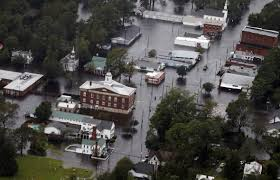
\includegraphics[height=0.4\textheight]{flood}
\end{frame}

\begin{frame}
\frametitle{40 most extreme temperature and precipitation events in the mid latitudes between 1979 and 2012.}
\centering
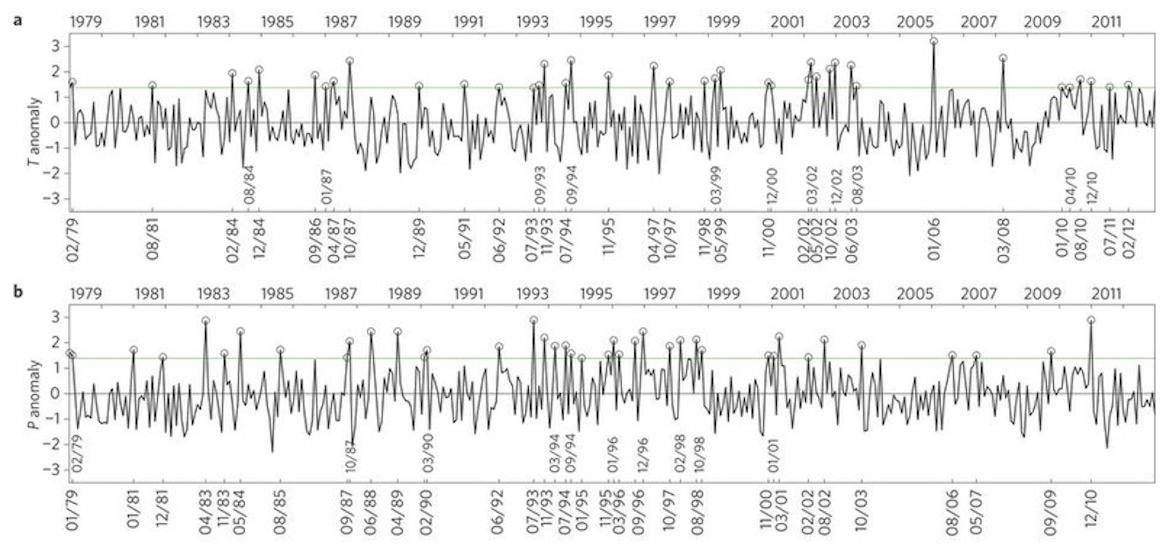
\includegraphics[scale=0.53]{Cathie1}


\end{frame}
\begin{frame}
\frametitle{Anomalies: Prolonged periods over a large area}
\begin{tabular}{c c}
\huge{Temperature}&\vspace{5pt}\\

\Large{Positive: abnormally high}	&	\Large{	Negative: abnormally low}\vspace{20pt}\\

\huge{Precipitation}&\vspace{5pt}\\
\Large{Positive: abnormally wet} &		\Large{	Negative: abnormally dry}\\
\end{tabular}


\end{frame}
\begin{frame}
\frametitle{Mid latitude regions of the Northern hemisphere examined}
\centering
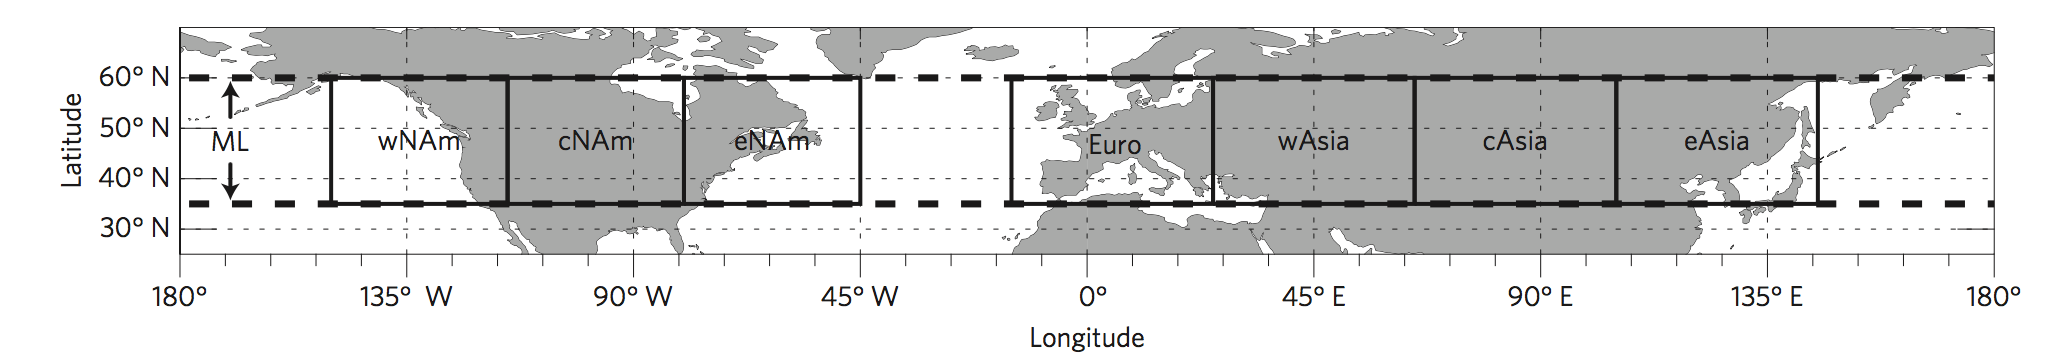
\includegraphics[scale=0.3]{Cathie2}
\end{frame}
\begin{frame}
\frametitle{Charts to show the normalized amplitude anomalies for each extreme temperature event, in order of severity of weather, taking the most extreme events on the left.}
\centering
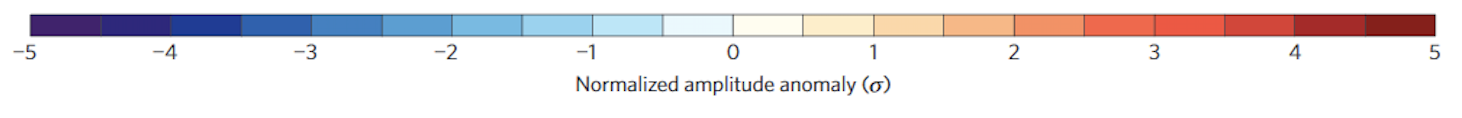
\includegraphics[scale=0.4]{Cathie4}
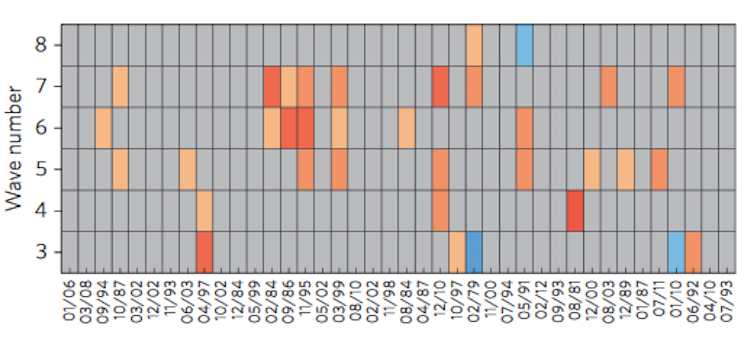
\includegraphics[scale=0.7]{Cathie5}
\end{frame}
\begin{frame}
\frametitle{Charts to show the normalized amplitude anomalies for each extreme precipitation event, in order of severity of weather, taking the most extreme events on the left.}
\centering
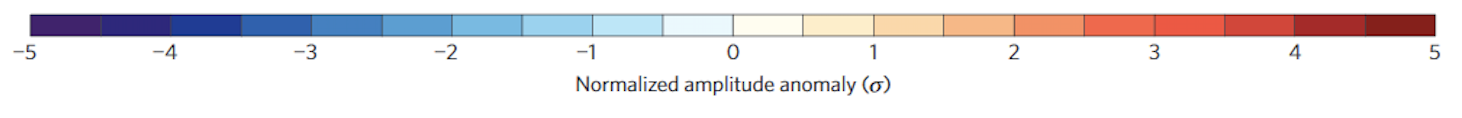
\includegraphics[scale=0.4]{Cathie4}
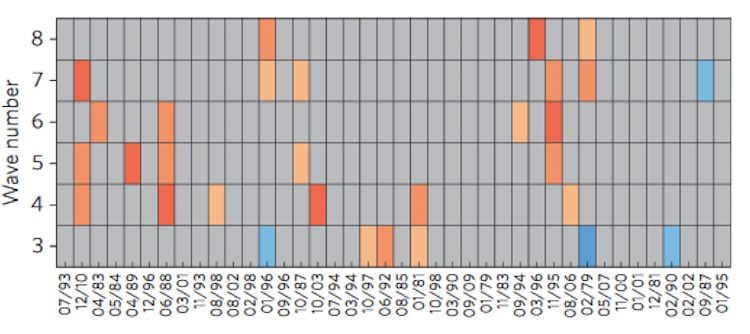
\includegraphics[scale=0.7]{Cathie6}
\end{frame}
\begin{frame}
\frametitle{Distributions comparing observed frequency of anomalous amplitudes of baroclinic Rossby waves during periods of extreme weather and the distributions expected from climatology across each examined region.}
\centering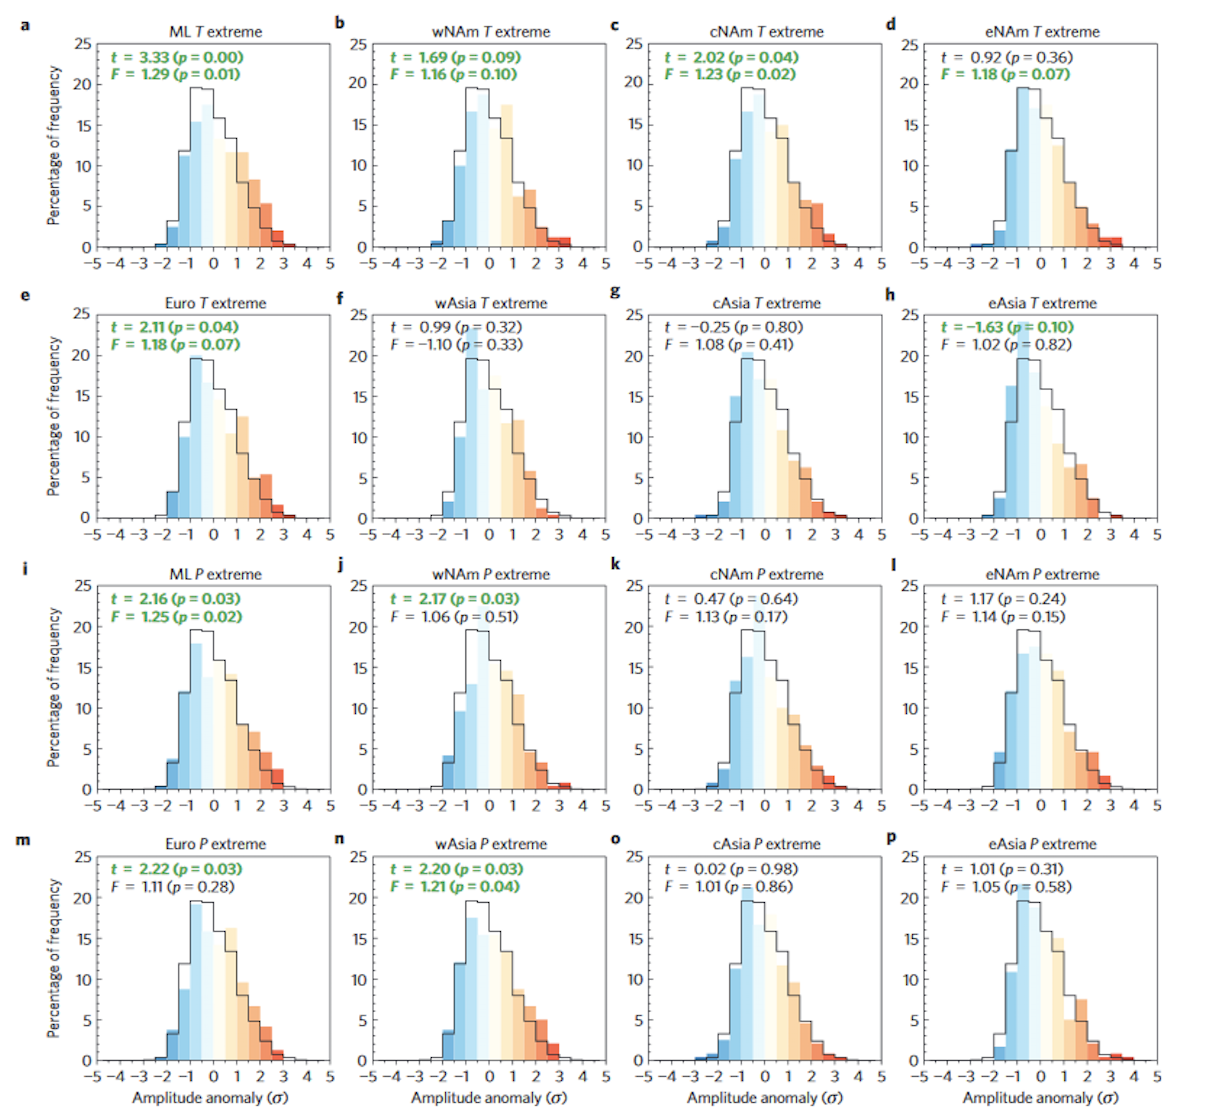
\includegraphics[scale=0.3]{Cathie7}
\end{frame}
\begin{frame}
\frametitle{Future Forecast}
\centering
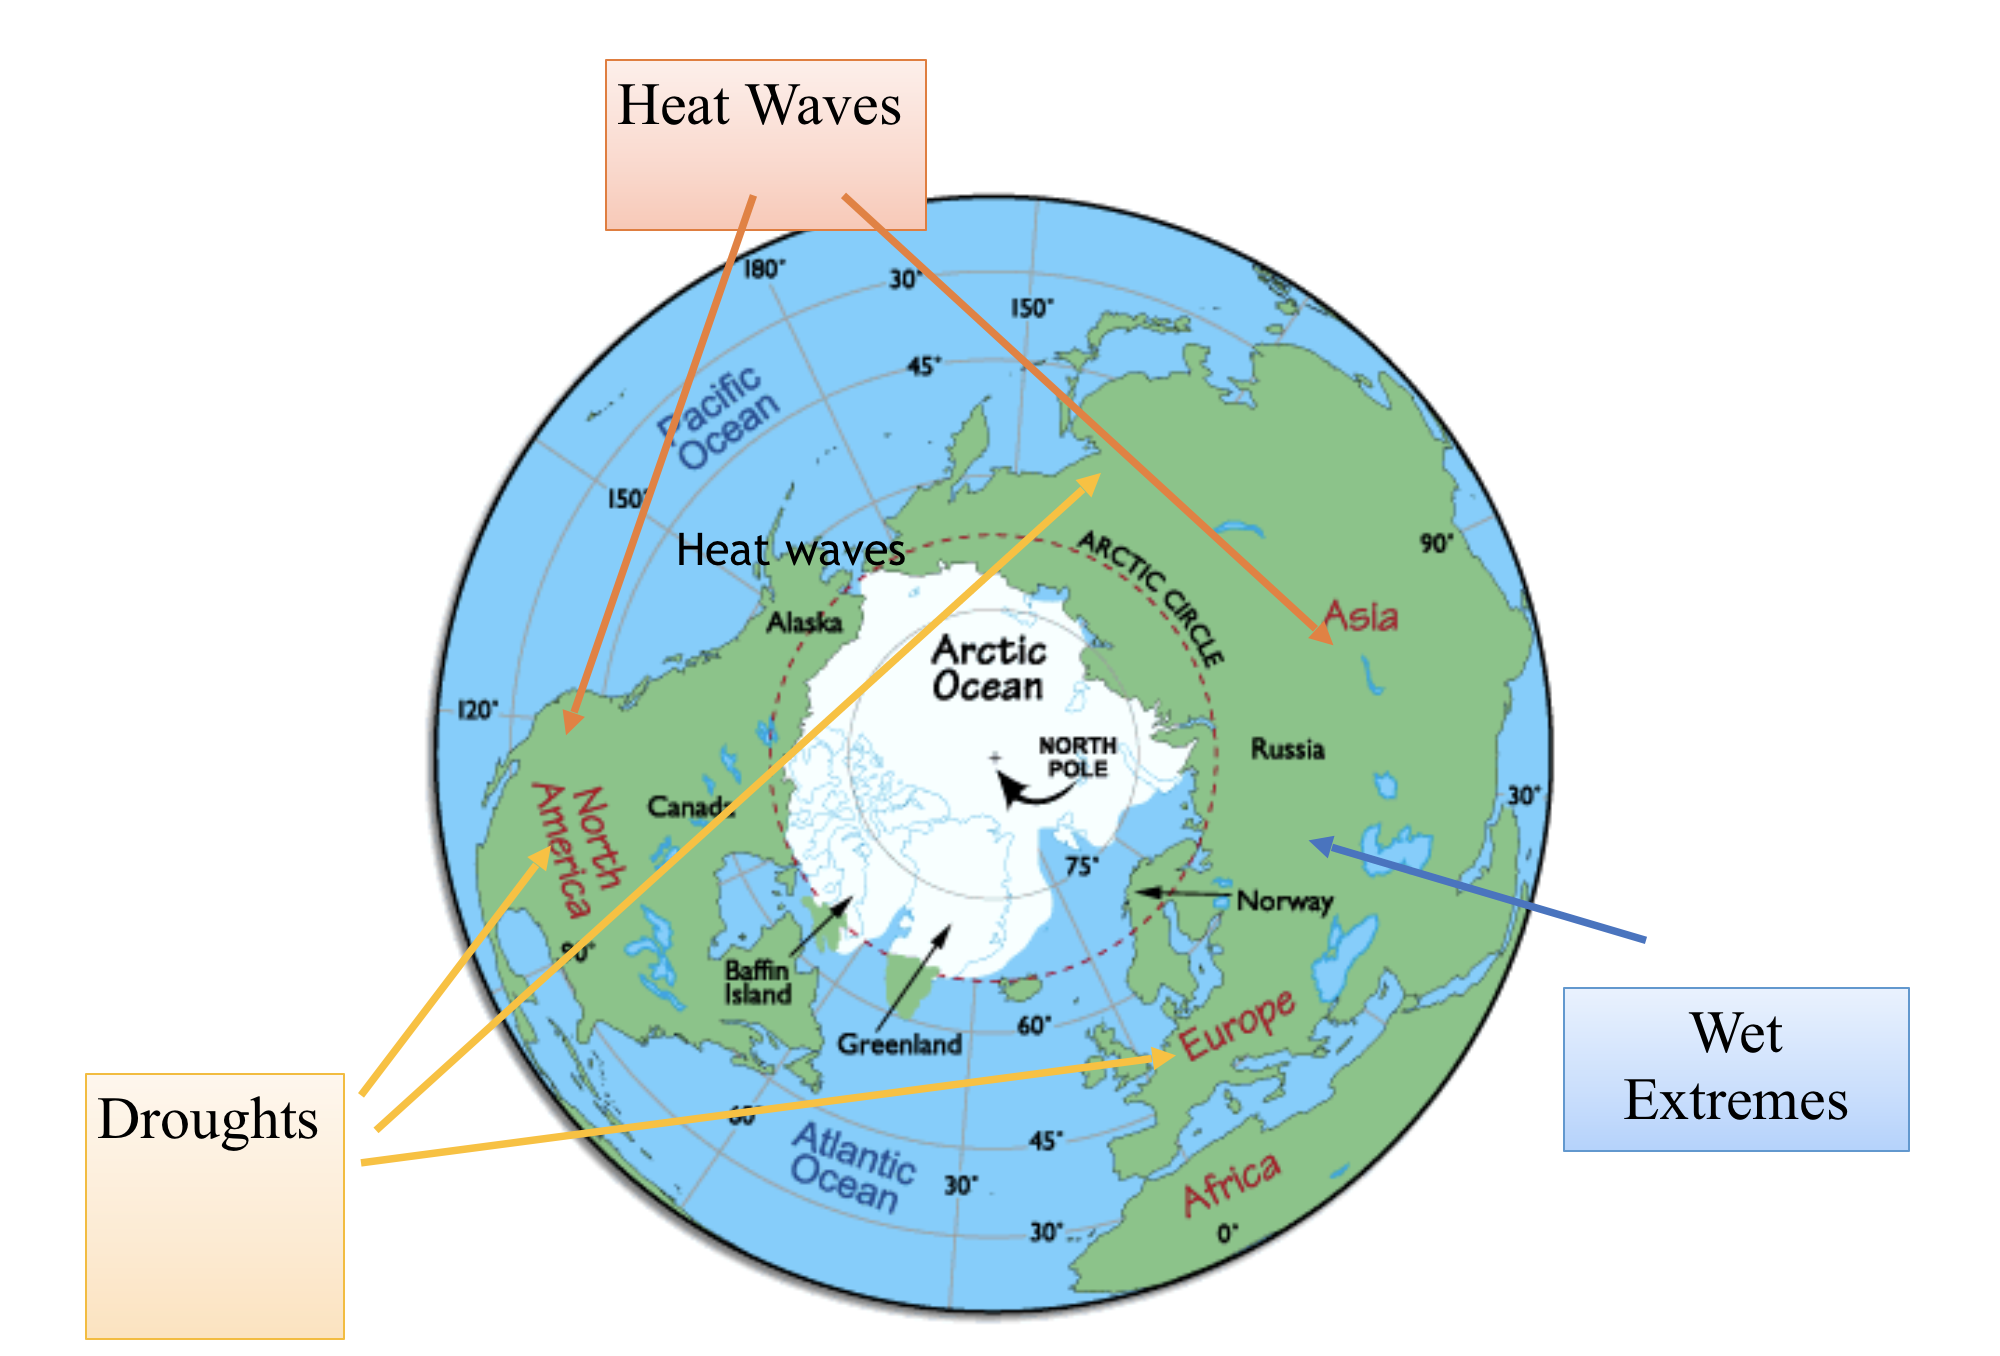
\includegraphics[scale=0.3]{Cathie8}

\end{frame}
\end{document}